\section{Hardware}
\label{sec:hw}

In this section we describe the hardware we used in the process of creating the device.

\subsection{Hardware Setup}
% TODO: čo bolo treba vytvoriť na sprovoznenie
% zapojenie arduino, raspberry
% popísať prečo je potreba arduino a púrečo je pi zlé (GPIO 3.3V vs 5V)
% schema konstrukcie / foto


\subsubsection*{Camera}
The selected camera is Basler raL6144-16gm. This camera provides us with the resolution of 6144 $\times$ 1 pixels with line rate up to 17 kHz. The captured image is in greyscale colors which for our use case is the desired output. The camera's shutter can be operated either via hardware or software trigger\footnote{The camera also disposes of "free-run mode".}.

The camera is equipped with AF Nikkor 50mm f1.8D lens. The lens suits our needs for multiple reason. It is relatively inexpensive, simple to use and has good depth-of-field control with aperture ranging from f/1.8 up to f/22.

\subsubsection*{Camera Mounting}
In order to acquire images with line camera either the object or camera has to move in smooth direct line. We decided to move the camera for various reason. The main reason is the human error. People can easily place a hand on a firm stable surface and keep the hand as it is for a long period of time, in our case no more than 30 seconds.

The camera is mounted on a slide rail with stepper motor with the platform facing down in order to mount the camera and light as seen in figure \ref{fig:rail}. The slide rail itself is mounted on an aluminium scaffolding which raises the rail to the desired height.

\begin{figure}[h]
    \label{fig:rail}
    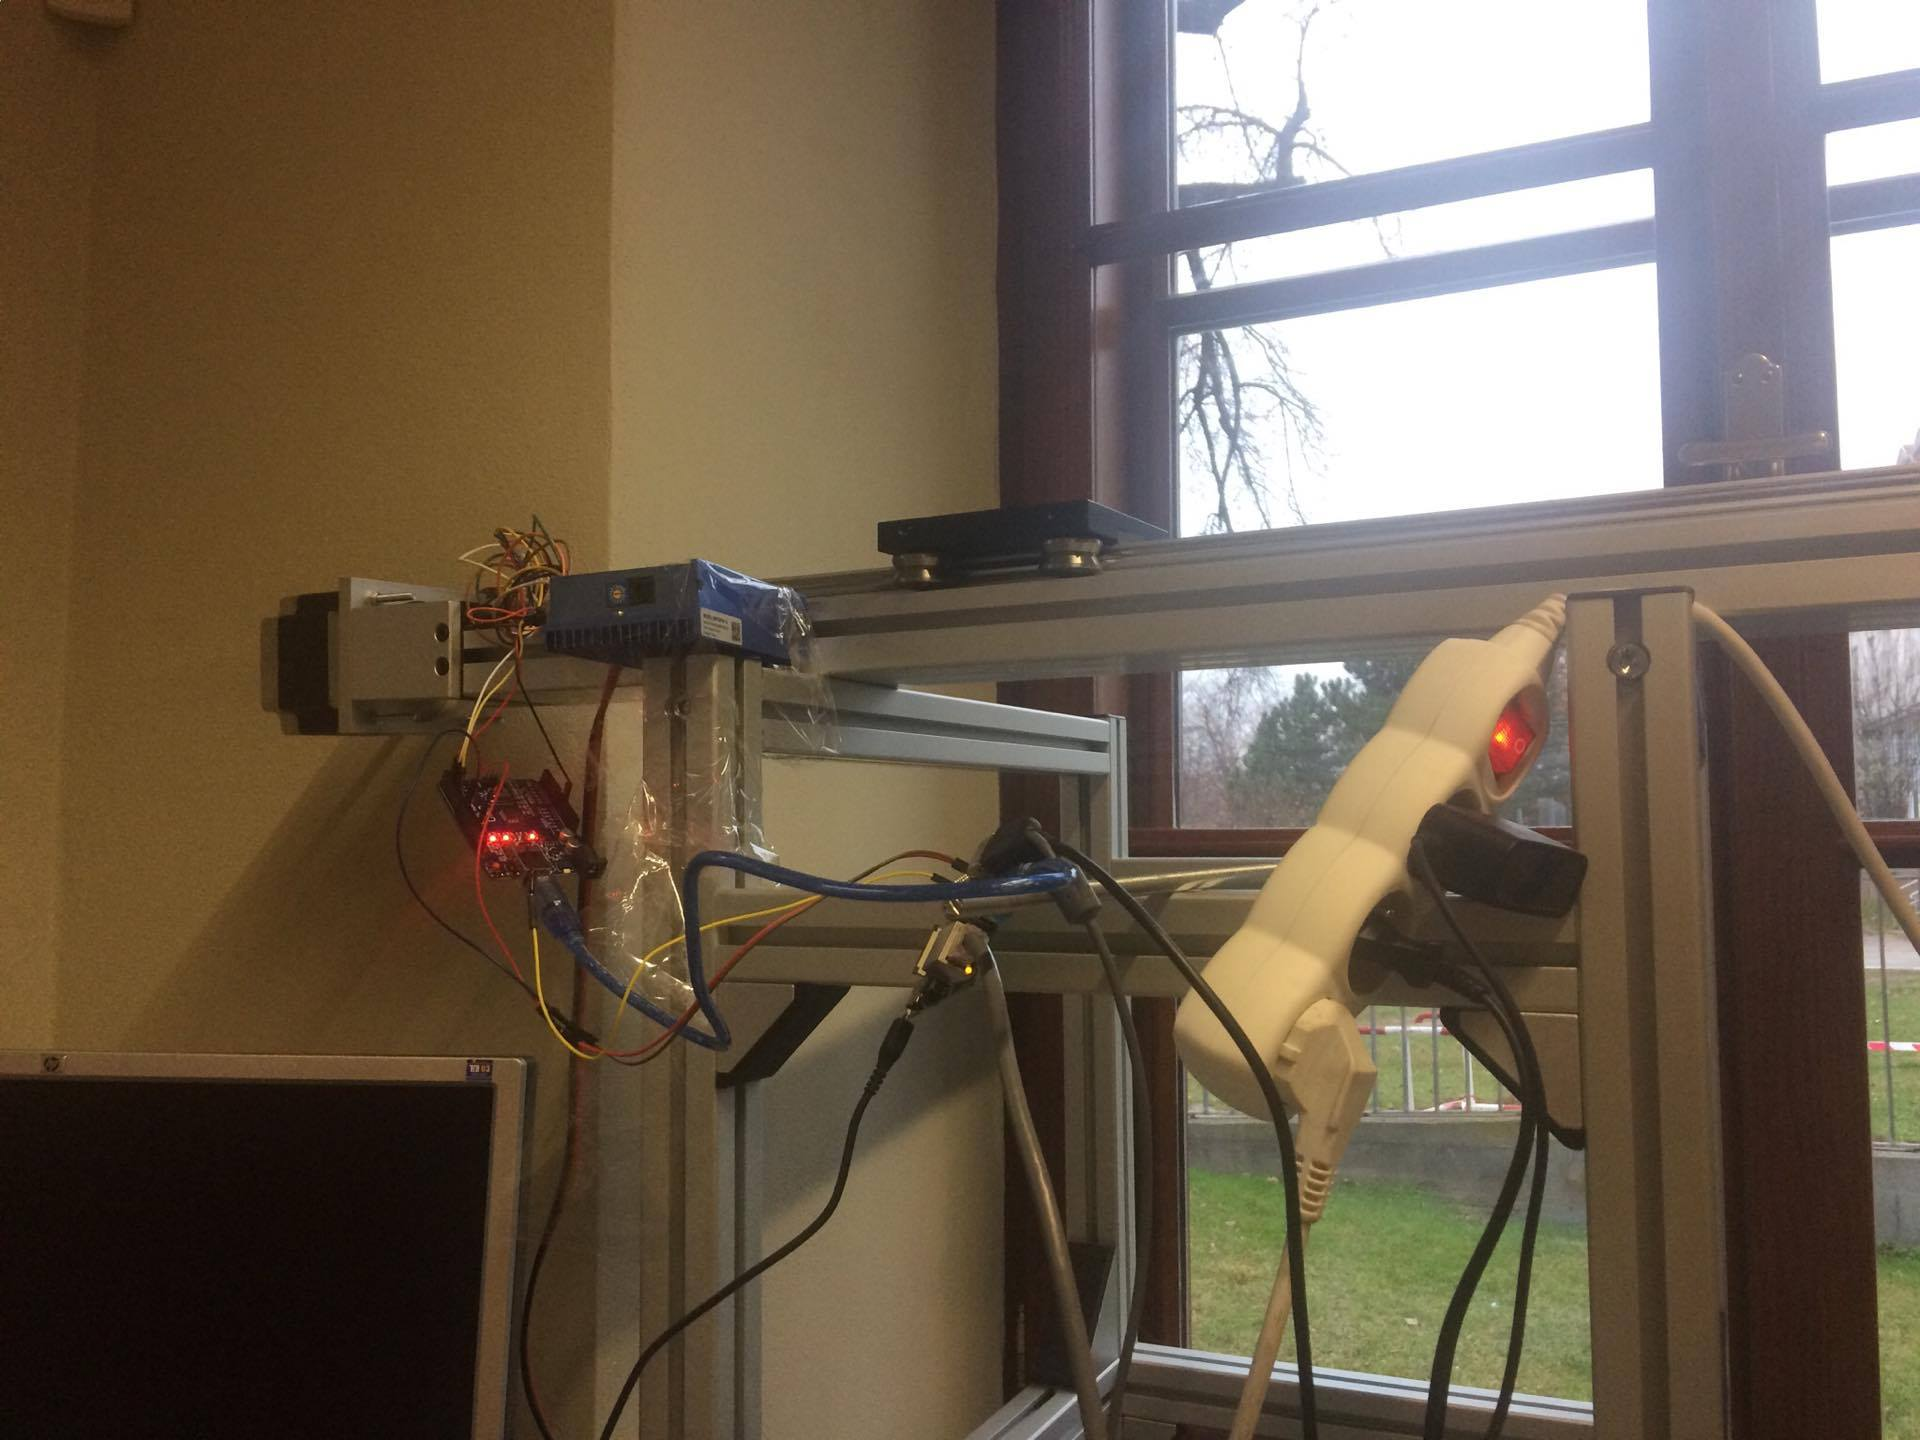
\includegraphics[width=\linewidth]{rail.jpg}
    \caption{Camera mount setup. ** tohle se jeste jednou vyfoti **}
\end{figure}

\subsubsection*{Slide Rail \& Stepper Motor}
We proposed for straight and smooth movement in one axis a slide rail controlled by a stepper motor. The stepper motor itself is controlled by Leadshine EM705 Digital Stepper Drive which is controlled by pulse width modulation generated by Arduino UNO with our custom code.

\subsection{Hand Placement}
The hand is placed in the centre of the scaffolding on a prepared foundation which aligns and spreads the fingers in order to always capture the same hand geometry. The hand stays put during the whole image acquisition procedure which minimizes the human error.

\begin{figure}[h]
    \label{fig:rail}
    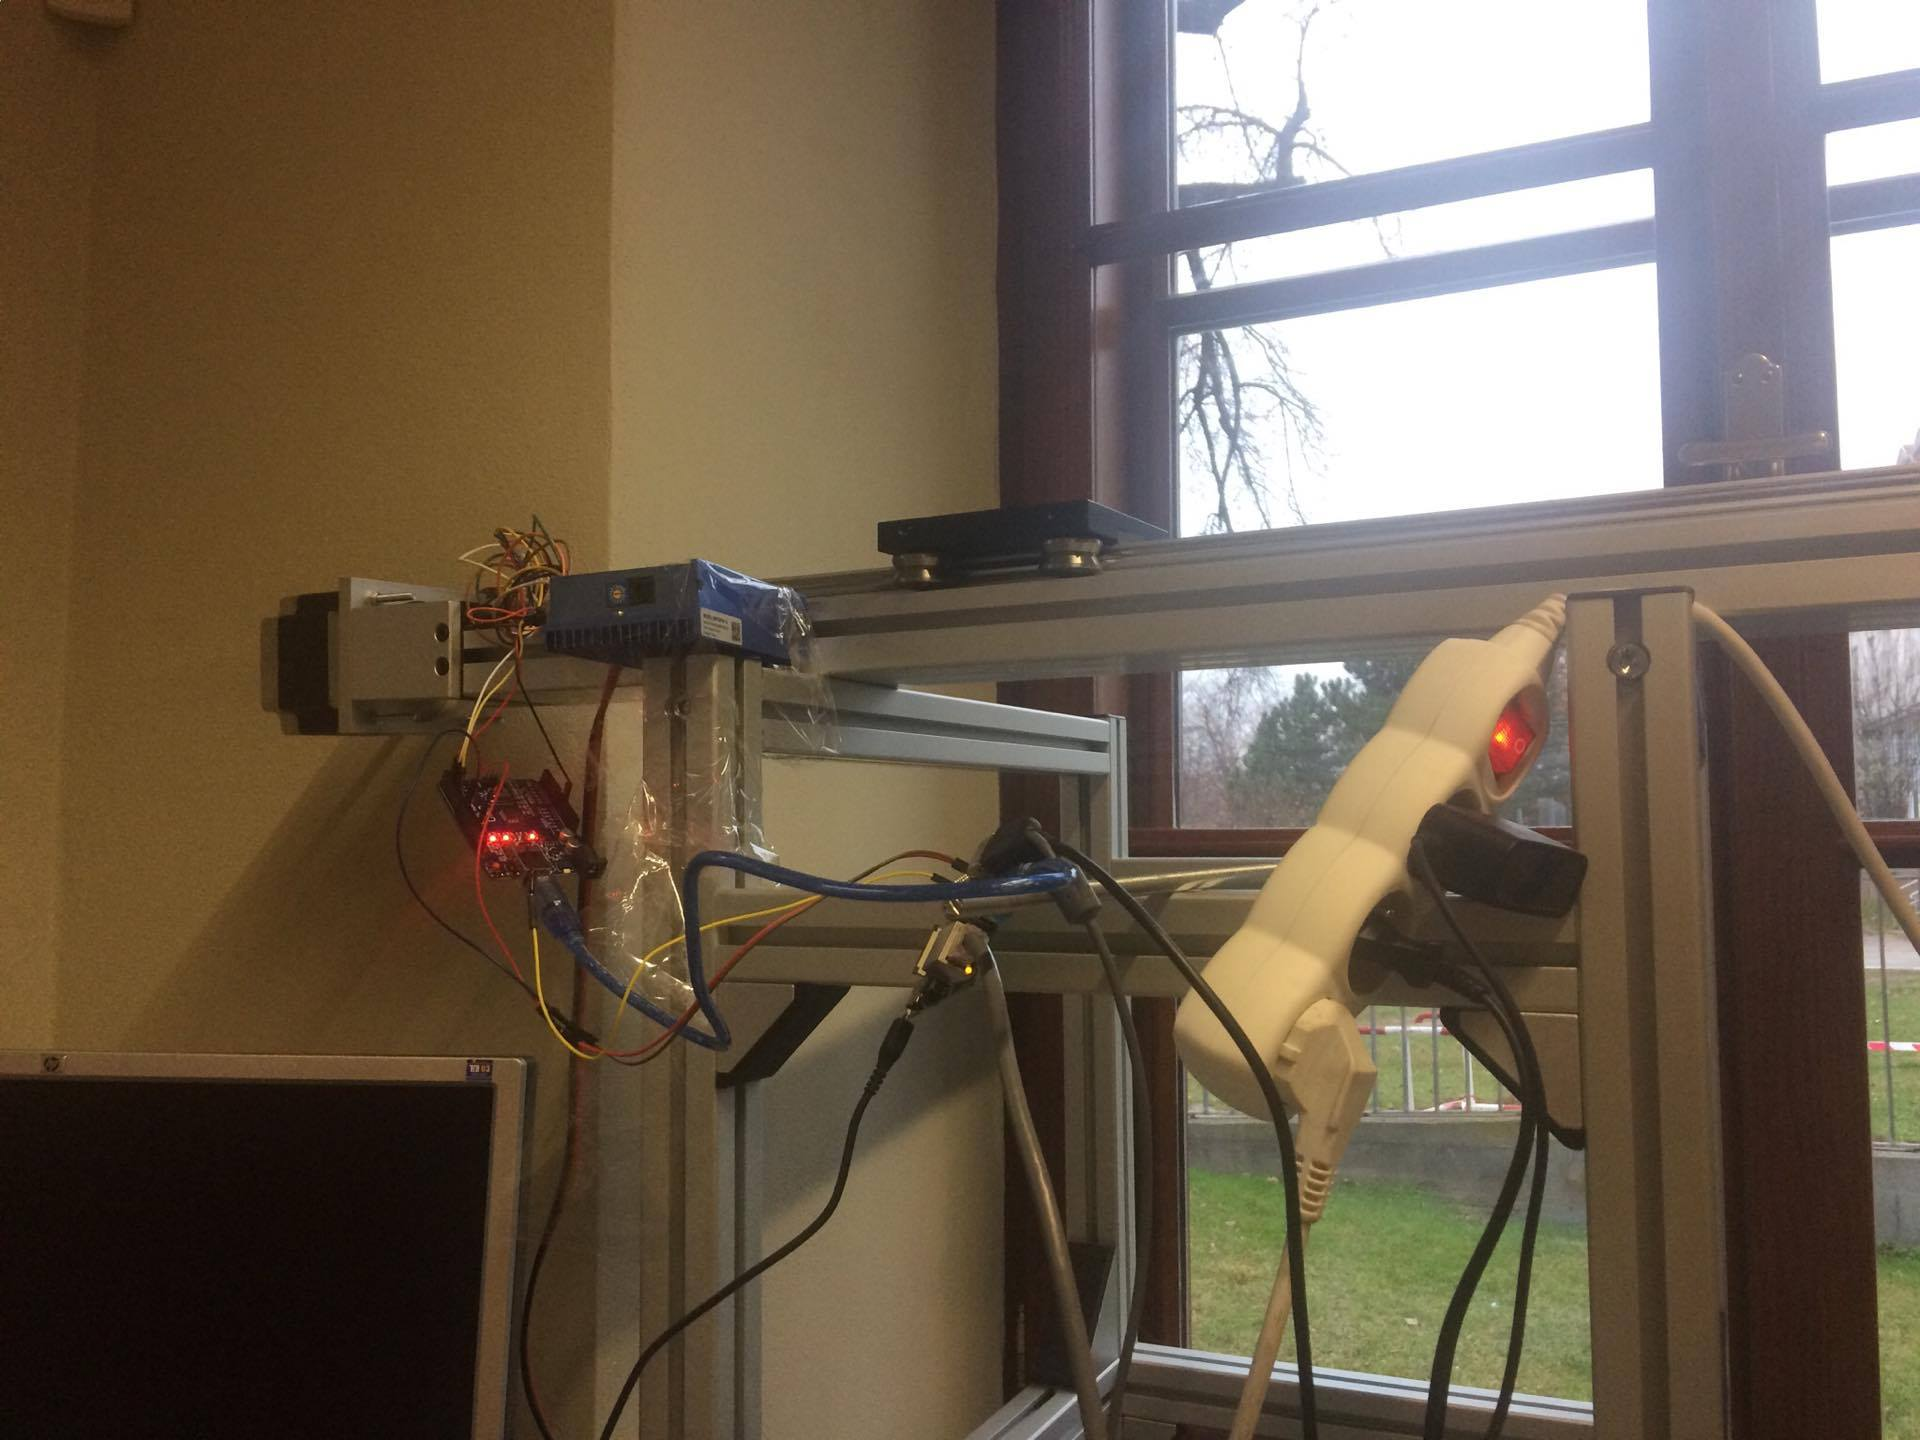
\includegraphics[width=0.5\linewidth]{rail.jpg}
    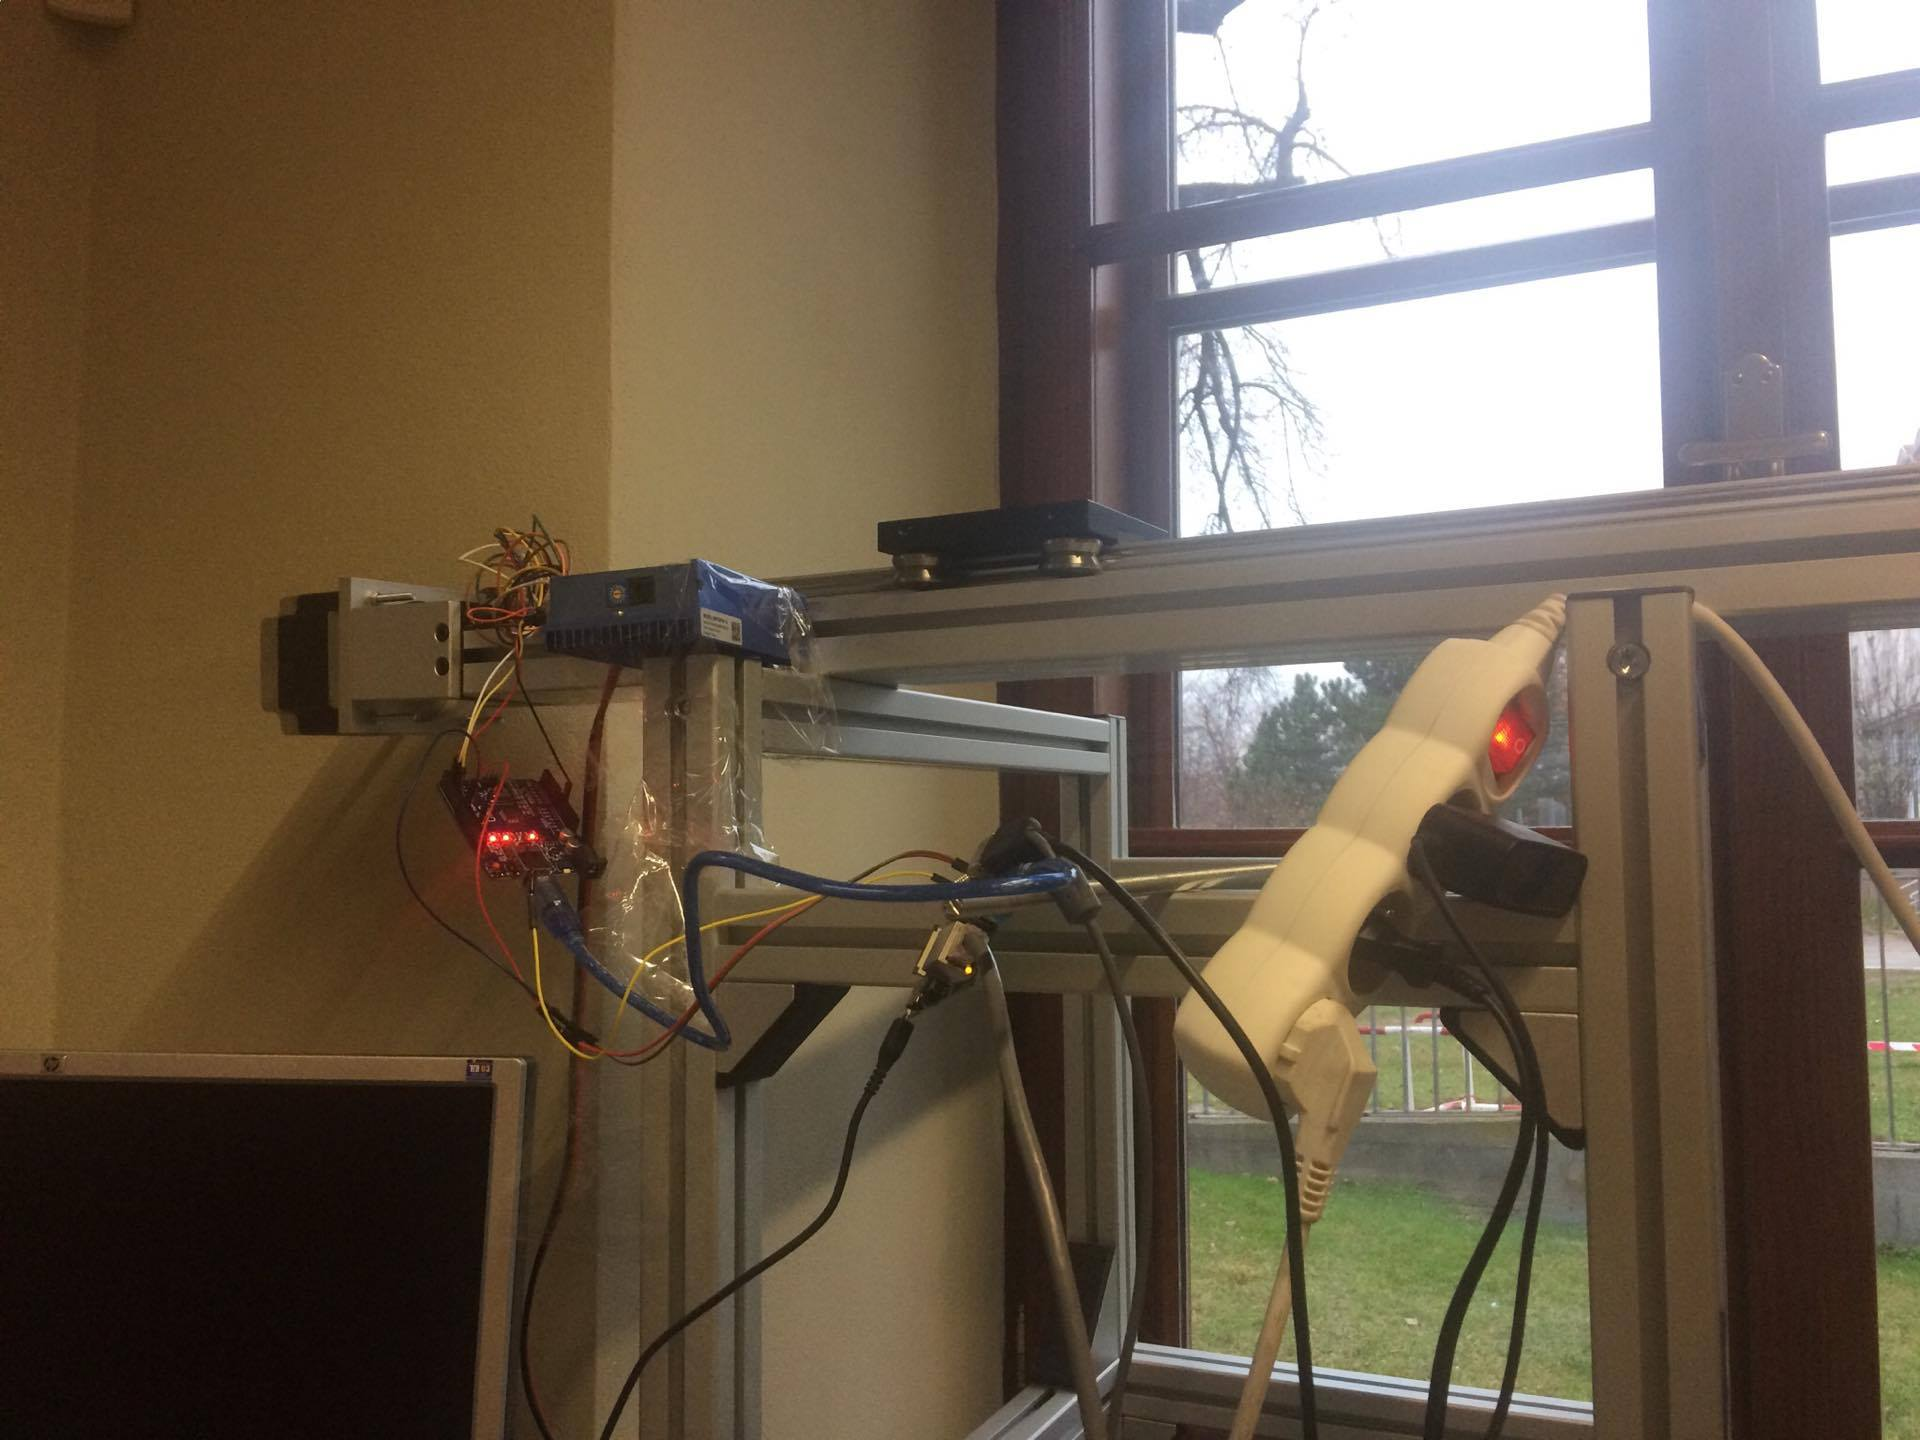
\includegraphics[width=0.5\linewidth]{rail.jpg}
    \caption{Tu bude neci ruka s deskou ** tohle se jeste jednou vyfoti **}
\end{figure}


\subsection{Slide Rail Control}
% TODO: nastavenie kontroleru - popisat problemy zo sekanim
% ako sme dospely k poctu sekund tam a s5 / pripadne vypocet vzorcom
Pohyb vozíka po koľajnici spočíva z jednosmerného pohybu stálou rýchlosťou vpravo, zastavení a opačného pohybu do pôvodnej pozície. \\
Pre pohyb vozíka je potrebná kontrola ovládacej jednotky motora, ktorý ovláda pohyb vozíka po koľajnici. Tento motor je ovládaný prostredníctvom Arduino UNO, ktoré prostredníctvom GPIO povoľuje pohyb a nastavuje smer pohybu. Pre ovládanie tejto fukcionality sa využíva ako kontrolér Raspberry Pi 3. Na raspberry beží program ktorý používa python program pre ovládanie GPIO pinov ktoré sú pripojené ku Arduino. Konkrétne sa využívajú výstupné GPIO piny:
\begin{itemize}
    \item PIN 18 - PWM
    \item PIN  5 - smer pohybu
    \item PIN  6 - povolenie pohybu
\end{itemize}


\subsection{Light Control}
\subsection{Camera Control}
%TODO: ako je ovladana kamera a prečo je to takto
% aka je vykonnost kamery a ake nastavenia prebehli
% ake je nastavenie osvetlenia -> pripadne samostatna sekcia o osvetleni
